\documentclass[tikz,border=12pt]{standalone}
\usepackage[T1]{fontenc}
\usepackage{mathpazo}
\usepackage{amsmath,amssymb}
\usetikzlibrary{arrows.meta, positioning, calc, fit, patterns}

\definecolor{stblue}{HTML}{7B97AD}
\definecolor{rwgold}{HTML}{B8995E}
\definecolor{sage}{HTML}{7A9A7E}
\definecolor{dkbrown}{HTML}{3D3530}
\definecolor{wmgray}{HTML}{7B7067}
\definecolor{cream}{HTML}{F9F6F0}
\definecolor{border}{HTML}{D4C9B8}
\definecolor{terracotta}{HTML}{C47A6A}
\definecolor{lavender}{HTML}{907EA0}

\begin{document}
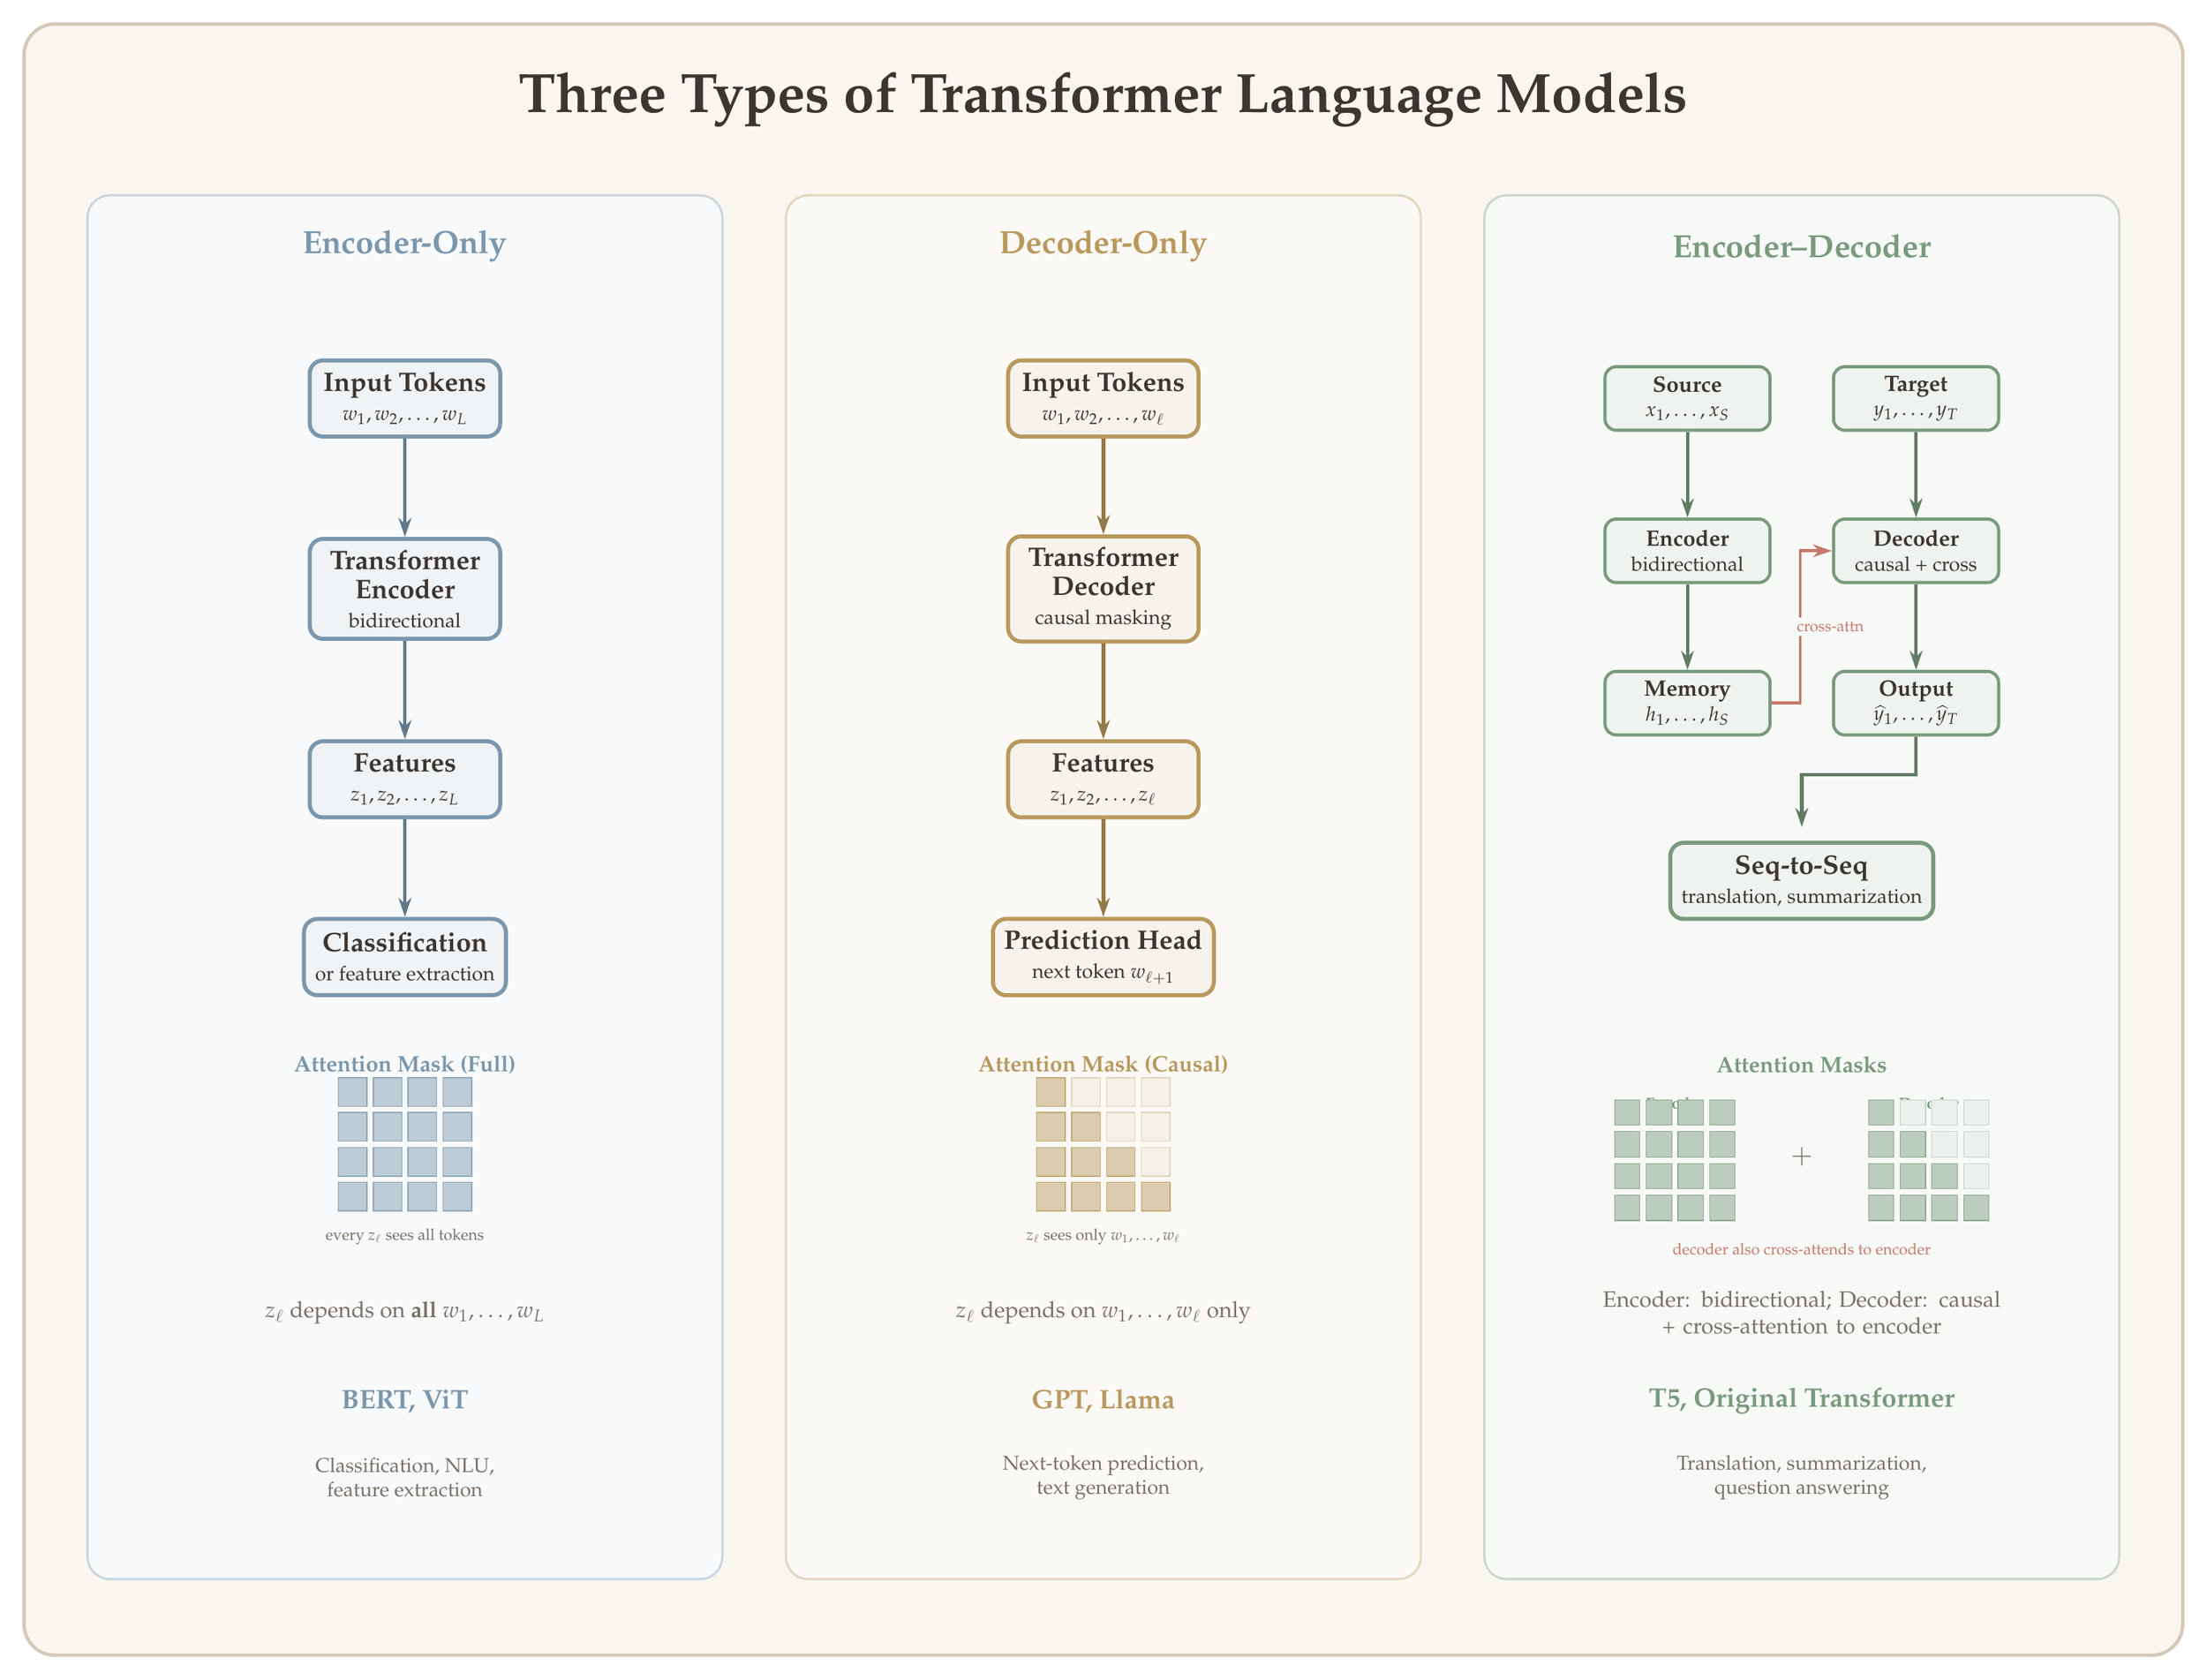
\begin{tikzpicture}[
  >={Stealth[length=3mm, width=2mm]},
  compbox/.style 2 args={
    draw=#1, line width=1.8pt, fill=#1!12, rounded corners=6pt,
    minimum width=30mm, minimum height=12mm, font=\large,
    text=dkbrown, align=center, inner sep=5pt
  },
  smallbox/.style 2 args={
    draw=#1, line width=1.4pt, fill=#1!12, rounded corners=5pt,
    minimum width=26mm, minimum height=10mm, font=\normalsize,
    text=dkbrown, align=center, inner sep=4pt
  },
  arr/.style={->, line width=1.6pt, dkbrown},
  note/.style={font=\small, text=wmgray, align=center},
  coltitle/.style={font=\Large\bfseries, text=dkbrown},
]

% ============================================================
% Background
% ============================================================
\fill[cream, rounded corners=14pt] (-1,-1.2) rectangle (33,24.5);
\draw[border, rounded corners=14pt, line width=1.5pt] (-1,-1.2) rectangle (33,24.5);

% Title
\node[font=\Huge\bfseries, text=dkbrown] at (16,23.3)
  {Three Types of Transformer Language Models};

% ============================================================
% Column backgrounds (subtle)
% ============================================================
\fill[stblue!6, rounded corners=10pt] (0, 0) rectangle (10, 21.8);
\draw[stblue!40, rounded corners=10pt, line width=1pt] (0, 0) rectangle (10, 21.8);

\fill[rwgold!6, rounded corners=10pt] (11, 0) rectangle (21, 21.8);
\draw[rwgold!40, rounded corners=10pt, line width=1pt] (11, 0) rectangle (21, 21.8);

\fill[sage!6, rounded corners=10pt] (22, 0) rectangle (32, 21.8);
\draw[sage!40, rounded corners=10pt, line width=1pt] (22, 0) rectangle (32, 21.8);

% ============================================================
% COLUMN 1: Encoder-Only (stblue)
% ============================================================
\def\colA{5}

% Title
\node[coltitle, text=stblue] at (\colA, 21)
  {Encoder-Only};

% --- Schematic ---
\node[compbox={stblue}{}] (inA) at (\colA, 18.6)
  {\textbf{Input Tokens}\\[-1pt]
   {\small $w_1, w_2, \ldots, w_L$}};

\node[compbox={stblue}{}] (encA) at (\colA, 15.6)
  {\textbf{Transformer}\\[-1pt]\textbf{Encoder}\\[-1pt]
   {\small bidirectional}};

\node[compbox={stblue}{}] (featA) at (\colA, 12.6)
  {\textbf{Features}\\[-1pt]
   {\small $z_1, z_2, \ldots, z_L$}};

\node[compbox={stblue}{}] (clsA) at (\colA, 9.8)
  {\textbf{Classification}\\[-1pt]
   {\small or feature extraction}};

\draw[arr, stblue!80!black] (inA.south) -- (encA.north);
\draw[arr, stblue!80!black] (encA.south) -- (featA.north);
\draw[arr, stblue!80!black] (featA.south) -- (clsA.north);

% --- Attention mask (full) ---
\node[font=\normalsize\bfseries, text=stblue] at (\colA, 8.1)
  {Attention Mask (Full)};

% Full attention grid: 4x4, all filled
\foreach \r in {0,...,3}{
  \foreach \c in {0,...,3}{
    \fill[stblue!50] (\colA-1.05+\c*0.55, 5.8+\r*0.55) rectangle ++(0.45,0.45);
    \draw[stblue!80, line width=0.5pt] (\colA-1.05+\c*0.55, 5.8+\r*0.55) rectangle ++(0.45,0.45);
  }
}
\node[font=\scriptsize, text=wmgray] at (\colA, 5.4) {every $z_\ell$ sees all tokens};

% --- Key property ---
\node[note, font=\normalsize] at (\colA, 4.2)
  {$z_\ell$ depends on \textbf{all} $w_1, \ldots, w_L$};

% --- Examples ---
\node[font=\large\bfseries, text=stblue] at (\colA, 2.8)
  {BERT, ViT};

% --- Task ---
\node[note] at (\colA, 1.6)
  {Classification, NLU,\\feature extraction};

% ============================================================
% COLUMN 2: Decoder-Only (rwgold)
% ============================================================
\def\colB{16}

% Title
\node[coltitle, text=rwgold] at (\colB, 21)
  {Decoder-Only};

% --- Schematic ---
\node[compbox={rwgold}{}] (inB) at (\colB, 18.6)
  {\textbf{Input Tokens}\\[-1pt]
   {\small $w_1, w_2, \ldots, w_\ell$}};

\node[compbox={rwgold}{}] (decB) at (\colB, 15.6)
  {\textbf{Transformer}\\[-1pt]\textbf{Decoder}\\[-1pt]
   {\small causal masking}};

\node[compbox={rwgold}{}] (featB) at (\colB, 12.6)
  {\textbf{Features}\\[-1pt]
   {\small $z_1, z_2, \ldots, z_\ell$}};

\node[compbox={rwgold}{}] (predB) at (\colB, 9.8)
  {\textbf{Prediction Head}\\[-1pt]
   {\small next token $w_{\ell+1}$}};

\draw[arr, rwgold!80!black] (inB.south) -- (decB.north);
\draw[arr, rwgold!80!black] (decB.south) -- (featB.north);
\draw[arr, rwgold!80!black] (featB.south) -- (predB.north);

% --- Attention mask (causal / lower-triangular) ---
\node[font=\normalsize\bfseries, text=rwgold] at (\colB, 8.1)
  {Attention Mask (Causal)};

% Lower-triangular attention grid: 4x4
\foreach \r in {0,...,3}{
  \foreach \c in {0,...,3}{
    \pgfmathtruncatemacro{\rr}{3-\r}
    \ifnum\c>\rr
      % unfilled (masked)
      \fill[rwgold!15] (\colB-1.05+\c*0.55, 5.8+\r*0.55) rectangle ++(0.45,0.45);
      \draw[rwgold!40, line width=0.5pt] (\colB-1.05+\c*0.55, 5.8+\r*0.55) rectangle ++(0.45,0.45);
    \else
      % filled (attended)
      \fill[rwgold!50] (\colB-1.05+\c*0.55, 5.8+\r*0.55) rectangle ++(0.45,0.45);
      \draw[rwgold!80, line width=0.5pt] (\colB-1.05+\c*0.55, 5.8+\r*0.55) rectangle ++(0.45,0.45);
    \fi
  }
}
\node[font=\scriptsize, text=wmgray] at (\colB, 5.4) {$z_\ell$ sees only $w_1, \ldots, w_\ell$};

% --- Key property ---
\node[note, font=\normalsize] at (\colB, 4.2)
  {$z_\ell$ depends on $w_1, \ldots, w_\ell$ only};

% --- Examples ---
\node[font=\large\bfseries, text=rwgold] at (\colB, 2.8)
  {GPT, Llama};

% --- Task ---
\node[note] at (\colB, 1.6)
  {Next-token prediction,\\text generation};

% ============================================================
% COLUMN 3: Encoder-Decoder (sage)
% ============================================================
\def\colC{27}

% Title
\node[coltitle, text=sage] at (\colC, 21)
  {Encoder--Decoder};

% --- Schematic (two sub-stacks side by side) ---
\def\colCL{25.2}
\def\colCR{28.8}

% Encoder side
\node[smallbox={sage}{}] (srcC) at (\colCL, 18.6)
  {\textbf{Source}\\[-1pt]
   {\small $x_1, \ldots, x_S$}};

\node[smallbox={sage}{}] (encC) at (\colCL, 16.2)
  {\textbf{Encoder}\\[-1pt]
   {\small bidirectional}};

\node[smallbox={sage}{}] (memC) at (\colCL, 13.8)
  {\textbf{Memory}\\[-1pt]
   {\small $h_1, \ldots, h_S$}};

\draw[arr, sage!80!black] (srcC.south) -- (encC.north);
\draw[arr, sage!80!black] (encC.south) -- (memC.north);

% Decoder side
\node[smallbox={sage}{}] (tgtC) at (\colCR, 18.6)
  {\textbf{Target}\\[-1pt]
   {\small $y_1, \ldots, y_T$}};

\node[smallbox={sage}{}] (decC) at (\colCR, 16.2)
  {\textbf{Decoder}\\[-1pt]
   {\small causal + cross}};

\node[smallbox={sage}{}] (outC) at (\colCR, 13.8)
  {\textbf{Output}\\[-1pt]
   {\small $\widehat{y}_1, \ldots, \widehat{y}_T$}};

\draw[arr, sage!80!black] (tgtC.south) -- (decC.north);
\draw[arr, sage!80!black] (decC.south) -- (outC.north);

% Cross-attention arrow: from memory east, jog right, then into decoder west
\draw[->, line width=1.4pt, terracotta]
  (memC.east) -- ++(0.45,0) |- (decC.west);
\node[font=\scriptsize, text=terracotta, fill=sage!6, inner sep=2pt]
  at ($(memC.east)!0.5!(decC.west) + (0.45, 0)$) {cross-attn};

% --- Task box ---
\node[compbox={sage}{}] (taskC) at (\colC, 11)
  {\textbf{Seq-to-Seq}\\[-1pt]
   {\small translation, summarization}};

% Arrow from Output down to Seq-to-Seq
\draw[arr, sage!80!black] (outC.south) -- ++(0,-0.6) -| (\colC, 11.85);

% --- Attention masks ---
\node[font=\normalsize\bfseries, text=sage] at (\colC, 8.1)
  {Attention Masks};

% Encoder mask (full) -- 4x4 on left
\node[font=\scriptsize\bfseries, text=sage] at (25, 7.5) {Encoder};
\foreach \r in {0,...,3}{
  \foreach \c in {0,...,3}{
    \fill[sage!50] (24.05+\c*0.5, 5.65+\r*0.5) rectangle ++(0.4,0.4);
    \draw[sage!80, line width=0.4pt] (24.05+\c*0.5, 5.65+\r*0.5) rectangle ++(0.4,0.4);
  }
}

% Plus sign between masks
\node[font=\large\bfseries, text=wmgray] at (27, 6.65) {$+$};

% Decoder mask (causal) -- 4x4 on right
\node[font=\scriptsize\bfseries, text=sage] at (29, 7.5) {Decoder};
\foreach \r in {0,...,3}{
  \foreach \c in {0,...,3}{
    \pgfmathtruncatemacro{\rr}{3-\r}
    \ifnum\c>\rr
      \fill[sage!15] (28.05+\c*0.5, 5.65+\r*0.5) rectangle ++(0.4,0.4);
      \draw[sage!40, line width=0.4pt] (28.05+\c*0.5, 5.65+\r*0.5) rectangle ++(0.4,0.4);
    \else
      \fill[sage!50] (28.05+\c*0.5, 5.65+\r*0.5) rectangle ++(0.4,0.4);
      \draw[sage!80, line width=0.4pt] (28.05+\c*0.5, 5.65+\r*0.5) rectangle ++(0.4,0.4);
    \fi
  }
}

% Cross-attention label below masks
\node[font=\scriptsize, text=terracotta] at (\colC, 5.2) {decoder also cross-attends to encoder};

% --- Key property ---
\node[note, font=\normalsize, text width=8cm] at (\colC, 4.2)
  {Encoder: bidirectional; Decoder: causal\\+ cross-attention to encoder};

% --- Examples ---
\node[font=\large\bfseries, text=sage] at (\colC, 2.8)
  {T5, Original Transformer};

% --- Task ---
\node[note] at (\colC, 1.6)
  {Translation, summarization,\\question answering};

\end{tikzpicture}
\end{document}
